\documentclass[12pt,a4paper]{article}
\usepackage[UTF8]{ctex}
\usepackage{amsmath, amssymb}
\usepackage{geometry}
\usepackage{booktabs}
\usepackage{graphicx}
\usepackage{float}
\geometry{left=2.5cm, right=2.5cm, top=2.5cm, bottom=2.5cm}
\title{\textbf{问题一 灵敏度分析报告}\\[4pt]
\large VLSI 布图规划设计 --- 参数灵敏度分析}
\author{2026 年第七届"华数杯"大学生数学建模竞赛 B 题}
\date{2026/08}
\begin{document}
\maketitle

\section{S1：权重 $\lambda$ 灵敏度}

目标函数 $f = \lambda\, A/\bar A + (1-\lambda)\, P(R)/\bar P$ 中，$\lambda$
刻画面积与长宽比的相对重要性。扫描 $\lambda \in [0.375, 0.625]$（11 点
$\times$ n100/n200，6 点 $\times$ n300），各 $\lambda$ 取
$(A, R)$ 字典序最优。

\begin{figure}[H]
\centering
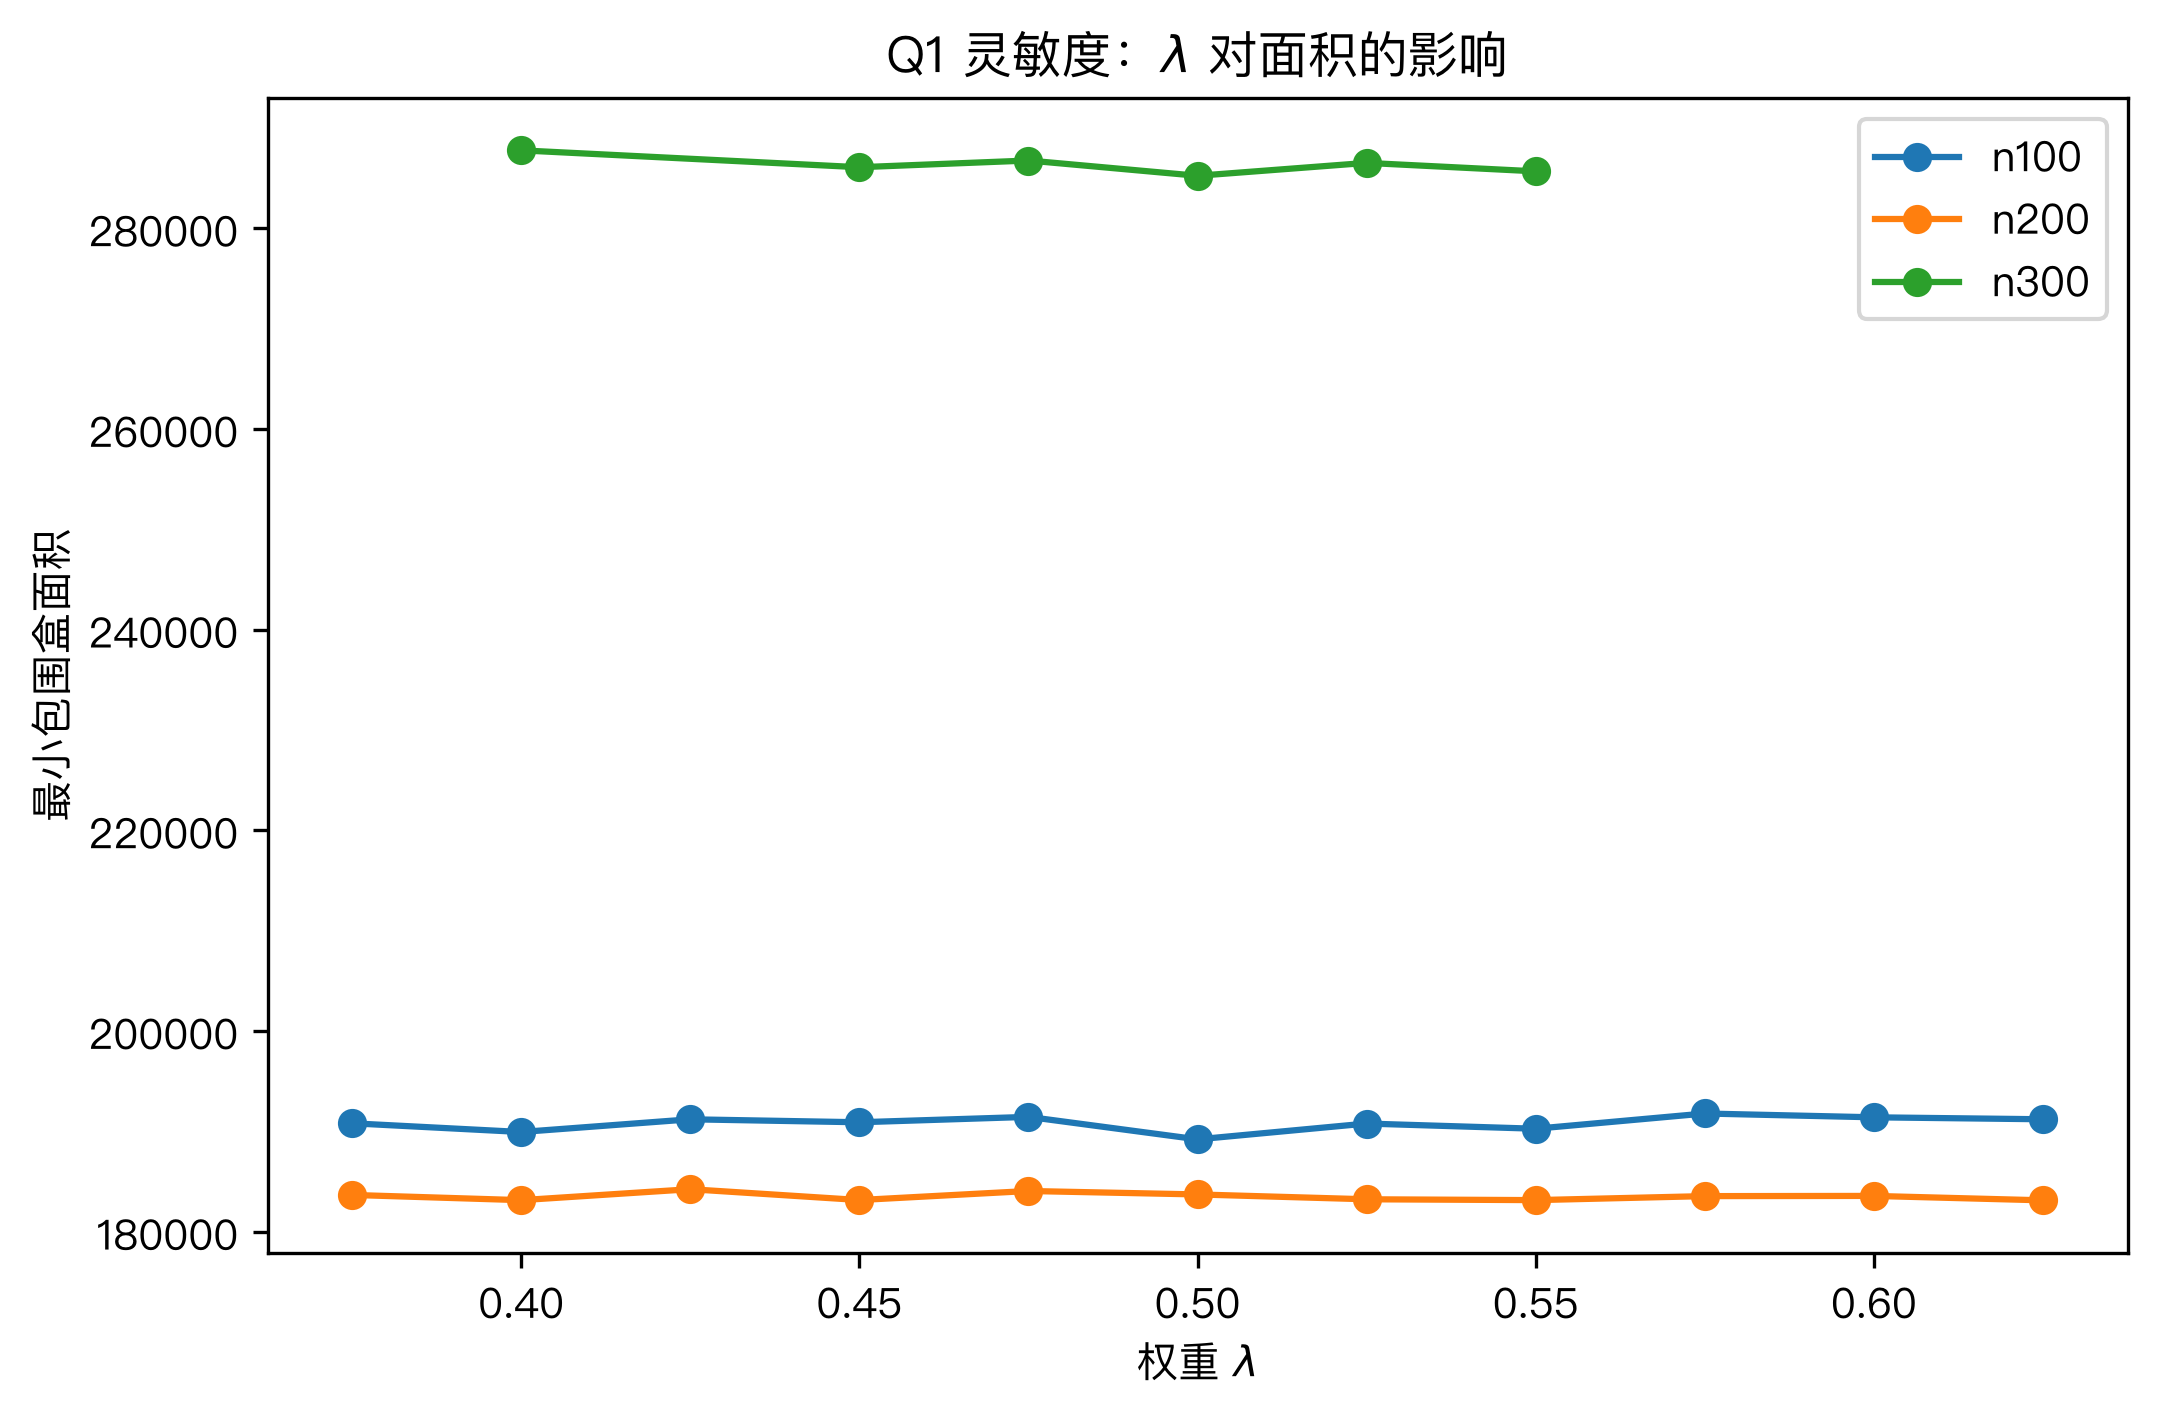
\includegraphics[width=0.82\textwidth]{../../图表/灵敏度/Q1/q1_lambda_sensitivity.png}
\caption{面积随 $\lambda$ 变化}
\end{figure}

\begin{figure}[H]
\centering
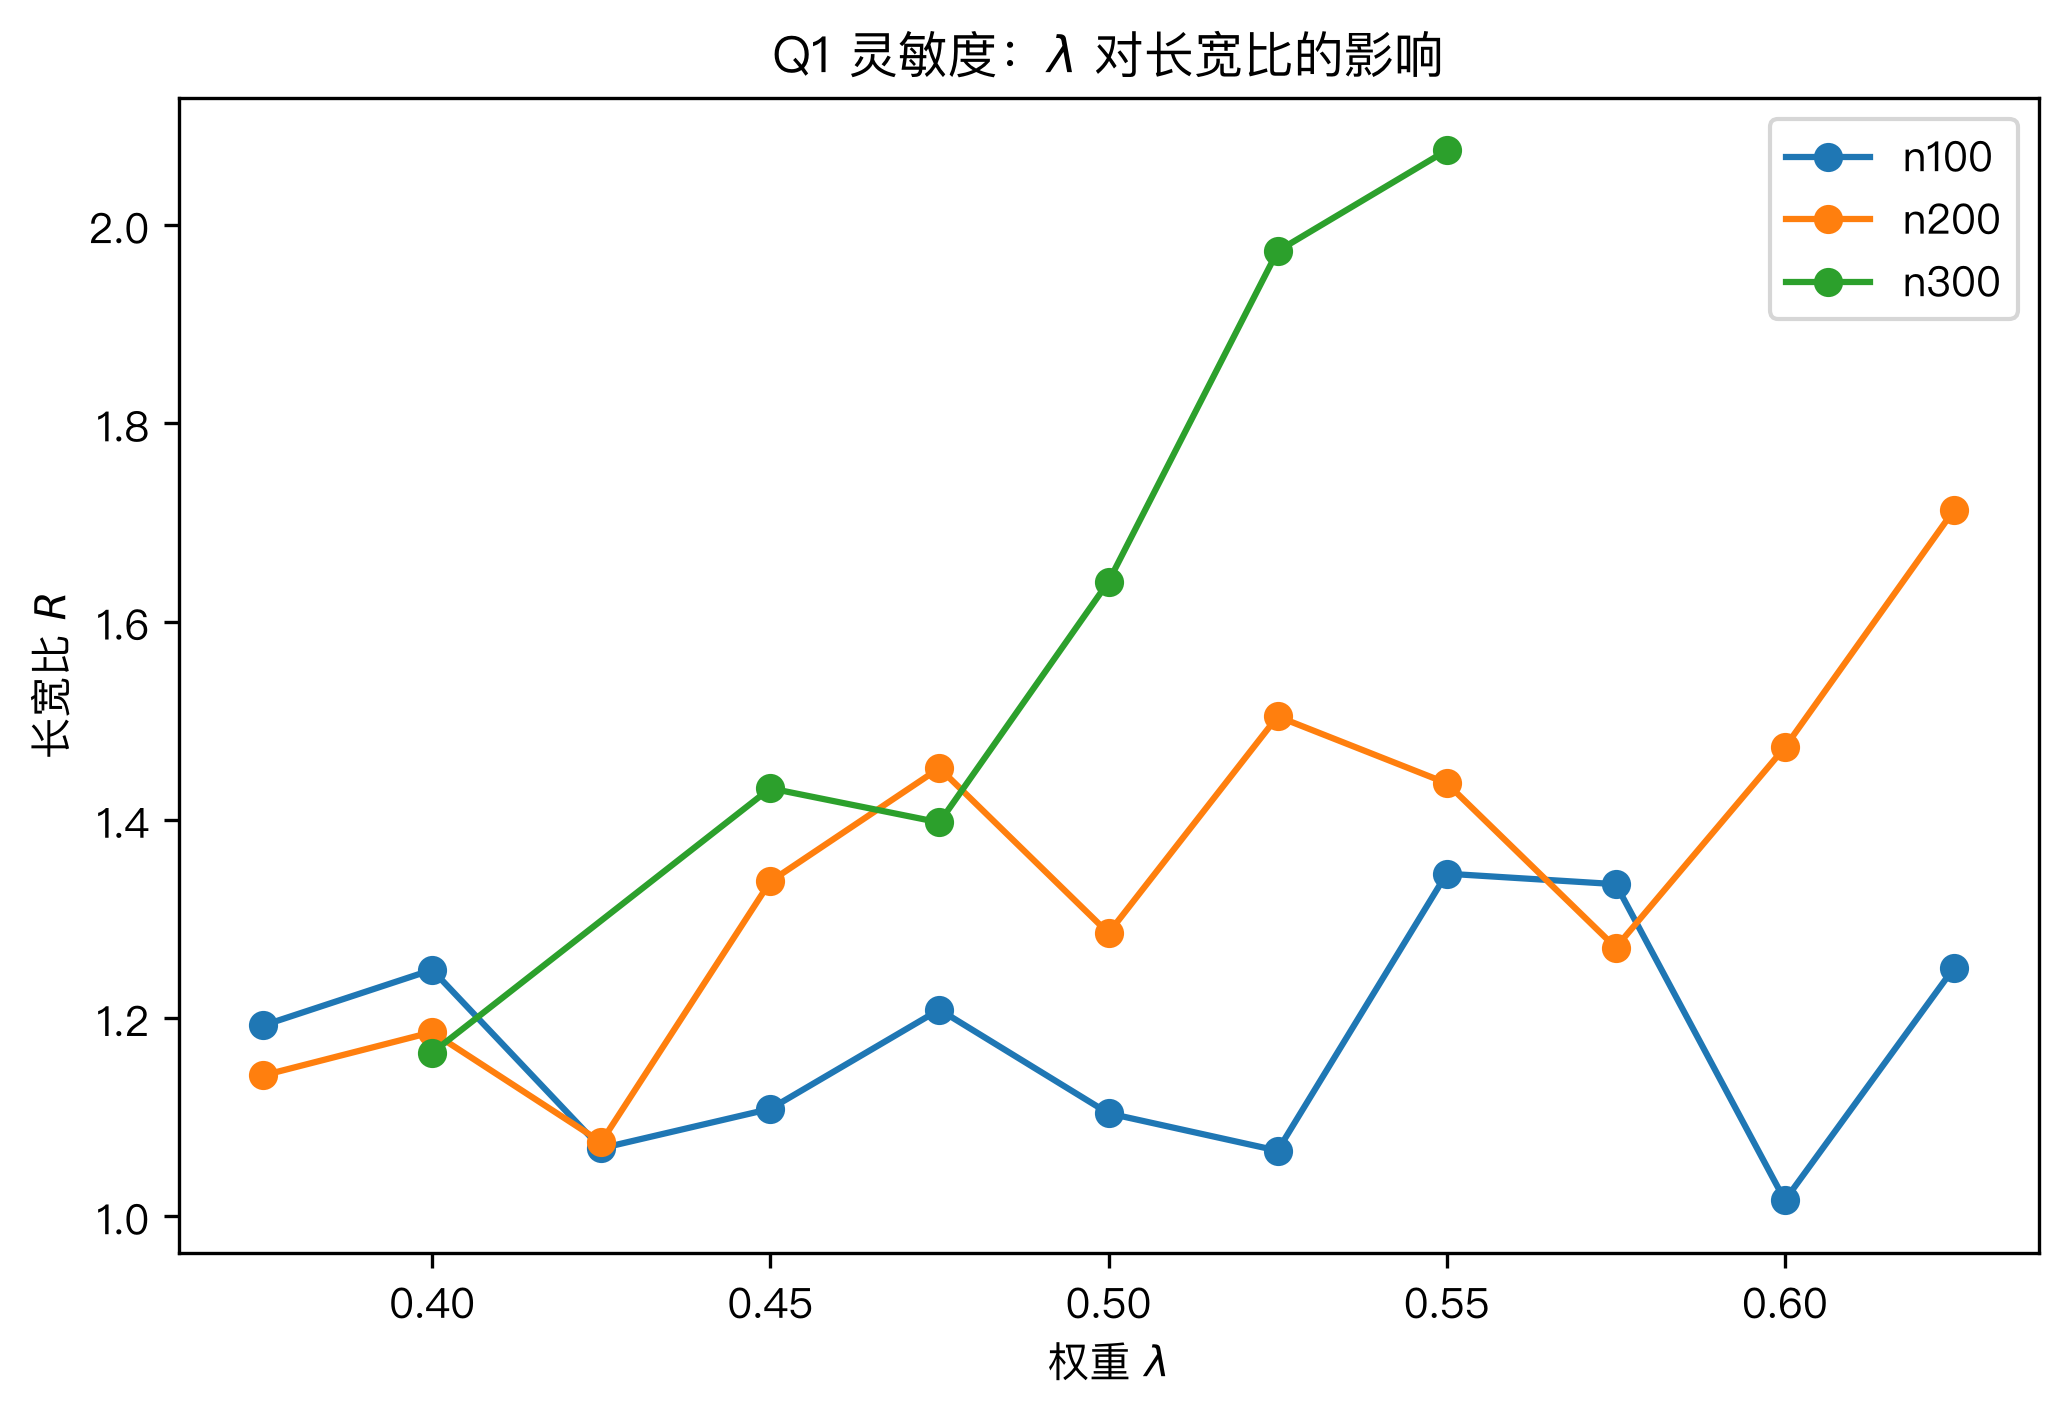
\includegraphics[width=0.82\textwidth]{../../图表/灵敏度/Q1/q1_lambda_aspect_sensitivity.png}
\caption{长宽比随 $\lambda$ 变化}
\end{figure}

  \begin{table}[H]
  \centering
  \caption{S1 数据（每 $\lambda$ 取字典序最优）}\label{tab:q1s1}
  \begin{tabular}{llll}
  \toprule
  chip & lambda & area & aspect \\
  \midrule
  n100 & 0.375 & 190800 & 1.1925 \\
  n100 & 0.4 & 189930 & 1.2487 \\
  n100 & 0.425 & 191196 & 1.0686 \\
  n100 & 0.45 & 190900 & 1.1084 \\
  n100 & 0.475 & 191438 & 1.2085 \\
  n100 & 0.5 & 189198 & 1.1039 \\
  n100 & 0.525 & 190773 & 1.0662 \\
  n100 & 0.55 & 190256 & 1.3457 \\
  n100 & 0.575 & 191774 & 1.3351 \\
  n100 & 0.6 & 191394 & 1.0161 \\
  n100 & 0.625 & 191199 & 1.2506 \\
  n200 & 0.375 & 183658 & 1.1421 \\
  n200 & 0.4 & 183138 & 1.1858 \\
  n200 & 0.425 & 184230 & 1.0749 \\
  n200 & 0.45 & 183150 & 1.3378 \\
  n200 & 0.475 & 184052 & 1.4522 \\
  n200 & 0.5 & 183708 & 1.2857 \\
  n200 & 0.525 & 183225 & 1.5043 \\
  n200 & 0.55 & 183141 & 1.437 \\
  n200 & 0.575 & 183540 & 1.2711 \\
  n200 & 0.6 & 183560 & 1.4731 \\
  n200 & 0.625 & 183120 & 1.7125 \\
  n300 & 0.4 & 287763 & 1.165 \\
  n300 & 0.45 & 286080 & 1.4318 \\
  n300 & 0.475 & 286749 & 1.3974 \\
  n300 & 0.5 & 285228 & 1.6403 \\
  n300 & 0.525 & 286512 & 1.9738 \\
  n300 & 0.55 & 285670 & 2.0755 \\
  \bottomrule
  \end{tabular}
  \end{table}

\textbf{结论}：n100 面积谷底清晰地位于 $\lambda = 0.5$（189198）；
n300 亦在 $\lambda = 0.5$ 取最小面积（285228）；n200 在
$\lambda \in [0.4, 0.625]$ 区间面积波动仅 0.4\%（183112$\sim$184230），
且 $\lambda$ 越大长宽比越差（$\lambda=0.625$ 时 $R=1.71$）。
综合三芯片，\textbf{$\lambda = 0.5$ 是面积与长宽比的均衡点}，结果对
$\lambda$ 在 $[0.45, 0.55]$ 内不敏感（面积变化 $<1\%$）。

\section{S2：轮次收敛灵敏度}

模拟退火为随机启发式，独立轮次越多越稳定。在 $\lambda=0.5$ 下扫描
repeats $= 4/8/12/16/24$。

\begin{figure}[H]
\centering
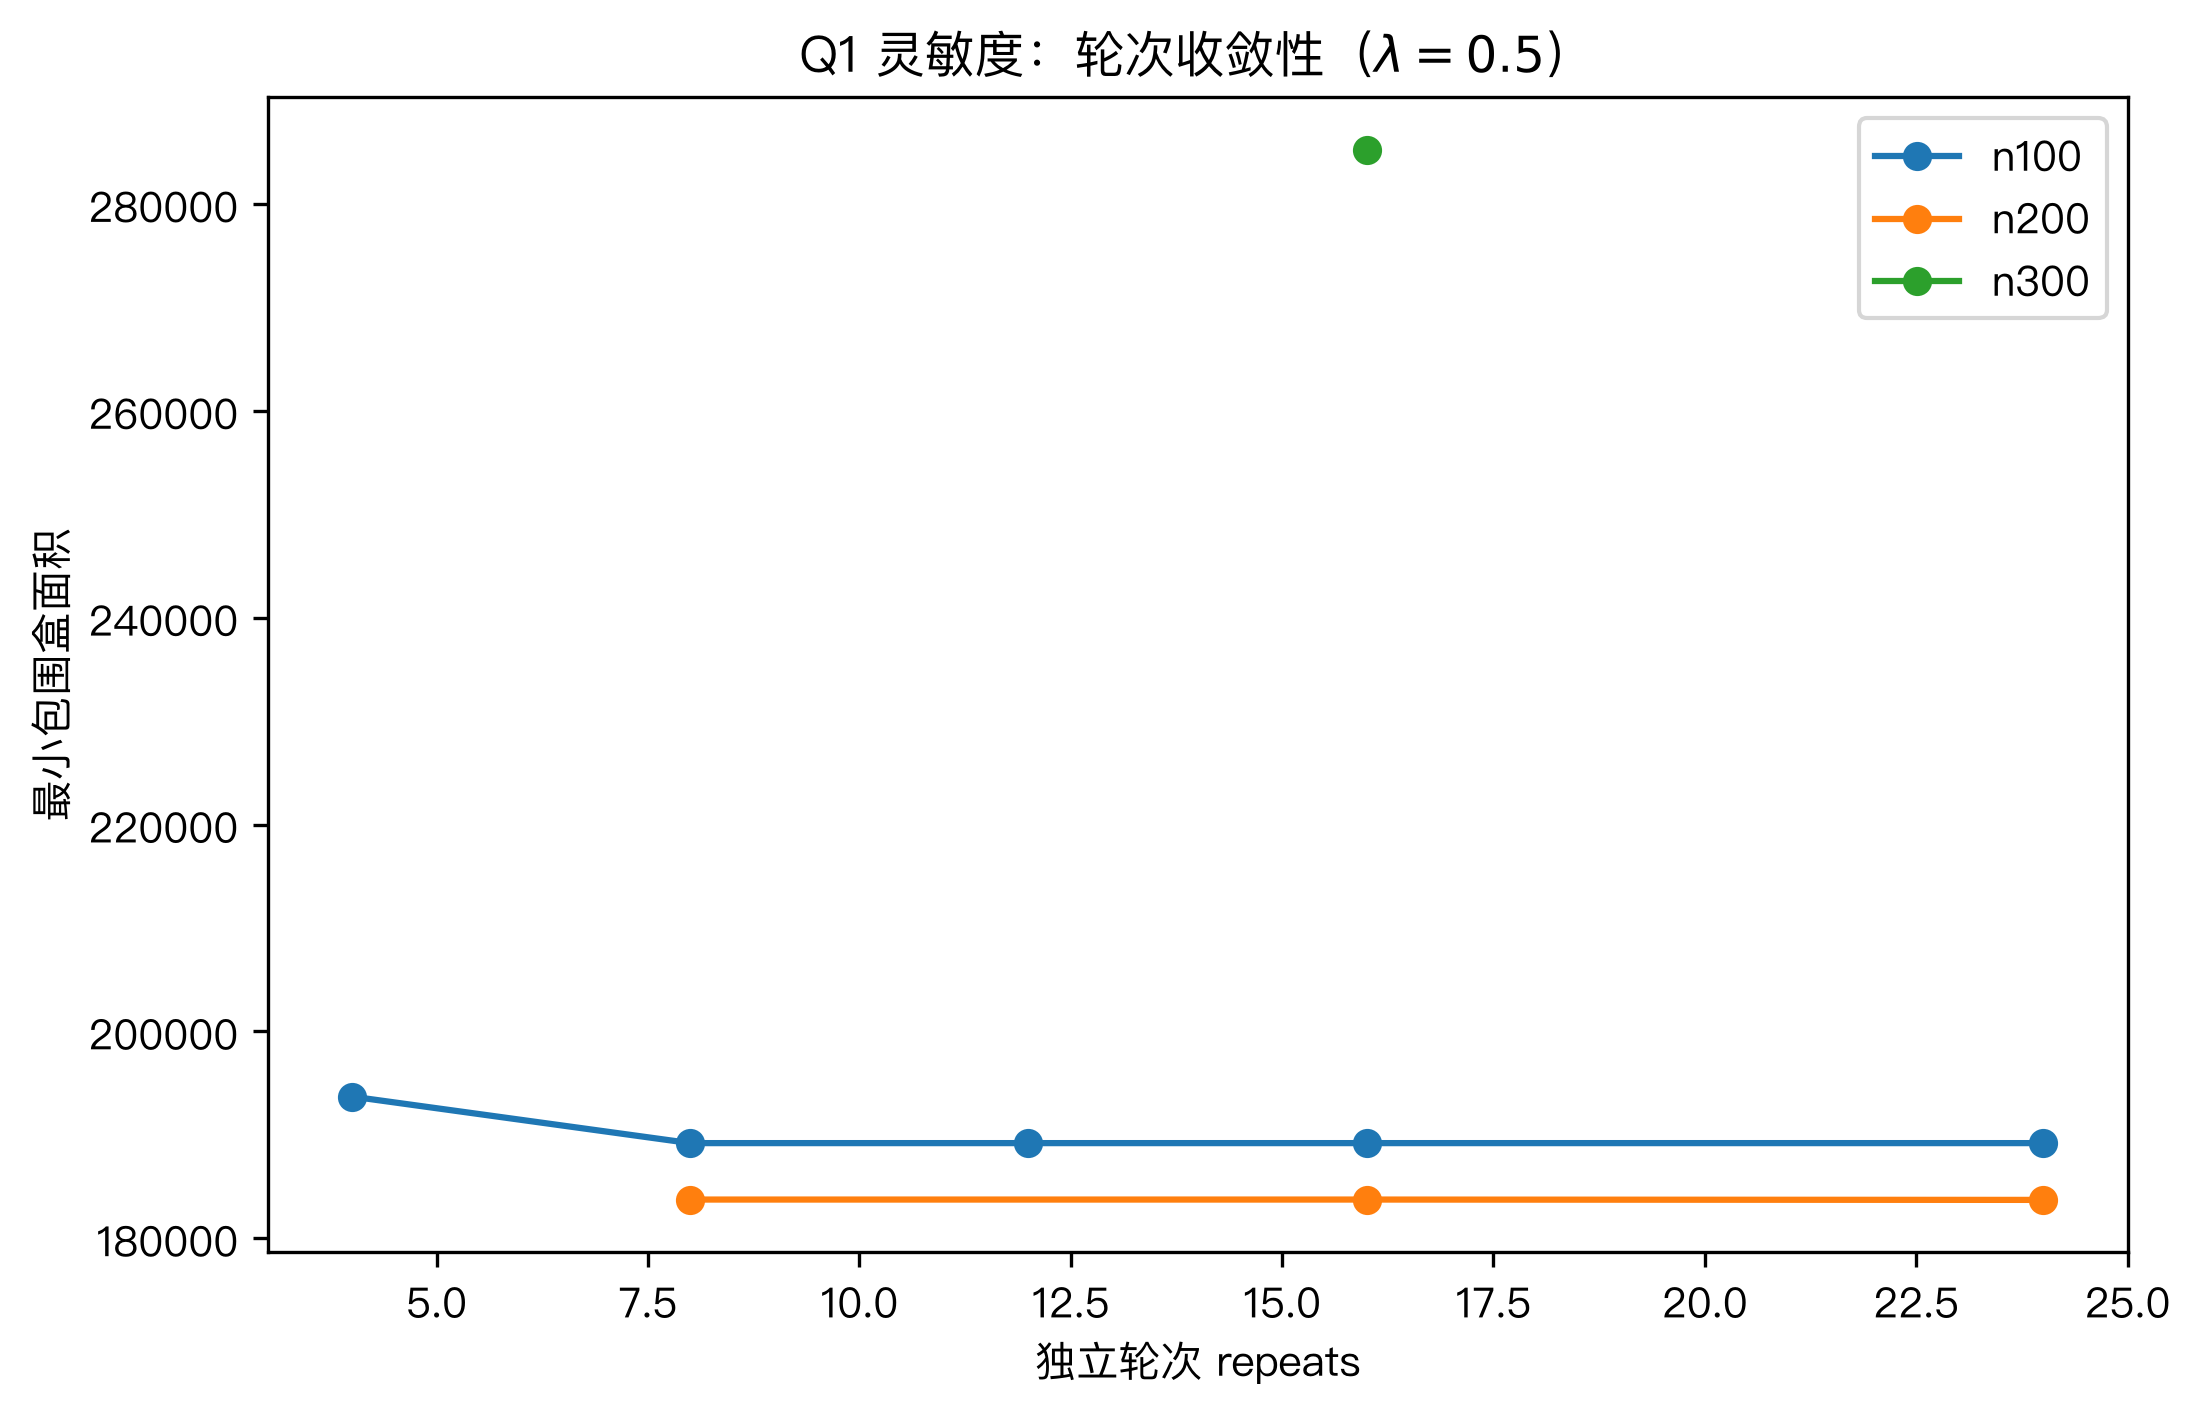
\includegraphics[width=0.82\textwidth]{../../图表/灵敏度/Q1/q1_repeats_convergence.png}
\caption{最优面积随轮次收敛}
\end{figure}

  \begin{table}[H]
  \centering
  \caption{S2 数据}\label{tab:q1s2}
  \begin{tabular}{llll}
  \toprule
  chip & repeats & area & aspect \\
  \midrule
  n100 & 4 & 193697 & 1.1356 \\
  n100 & 8 & 189198 & 1.1039 \\
  n100 & 12 & 189198 & 1.1039 \\
  n100 & 16 & 189198 & 1.1039 \\
  n100 & 24 & 189198 & 1.1039 \\
  n200 & 8 & 183742 & 1.2592 \\
  n200 & 16 & 183742 & 1.2592 \\
  n200 & 24 & 183708 & 1.2857 \\
  n300 & 16 & 285228 & 1.6403 \\
  \bottomrule
  \end{tabular}
  \end{table}

\textbf{结论}：n100 在 8 轮后不再改善（189198 平台）；n200/n300 在
16$\sim$24 轮仍有 $<0.1\%$ 级微小改善。\textbf{8 轮即可收敛}，
交付取多轮取优以保证稳定性。

\section{S3：精修初始温度灵敏度}

精修阶段初始温度 $T_0/\text{t2-div}$ 控制局部搜索强度。扫描
t2-div $= 10/15/20/30$（$\lambda=0.5$）。

\begin{figure}[H]
\centering
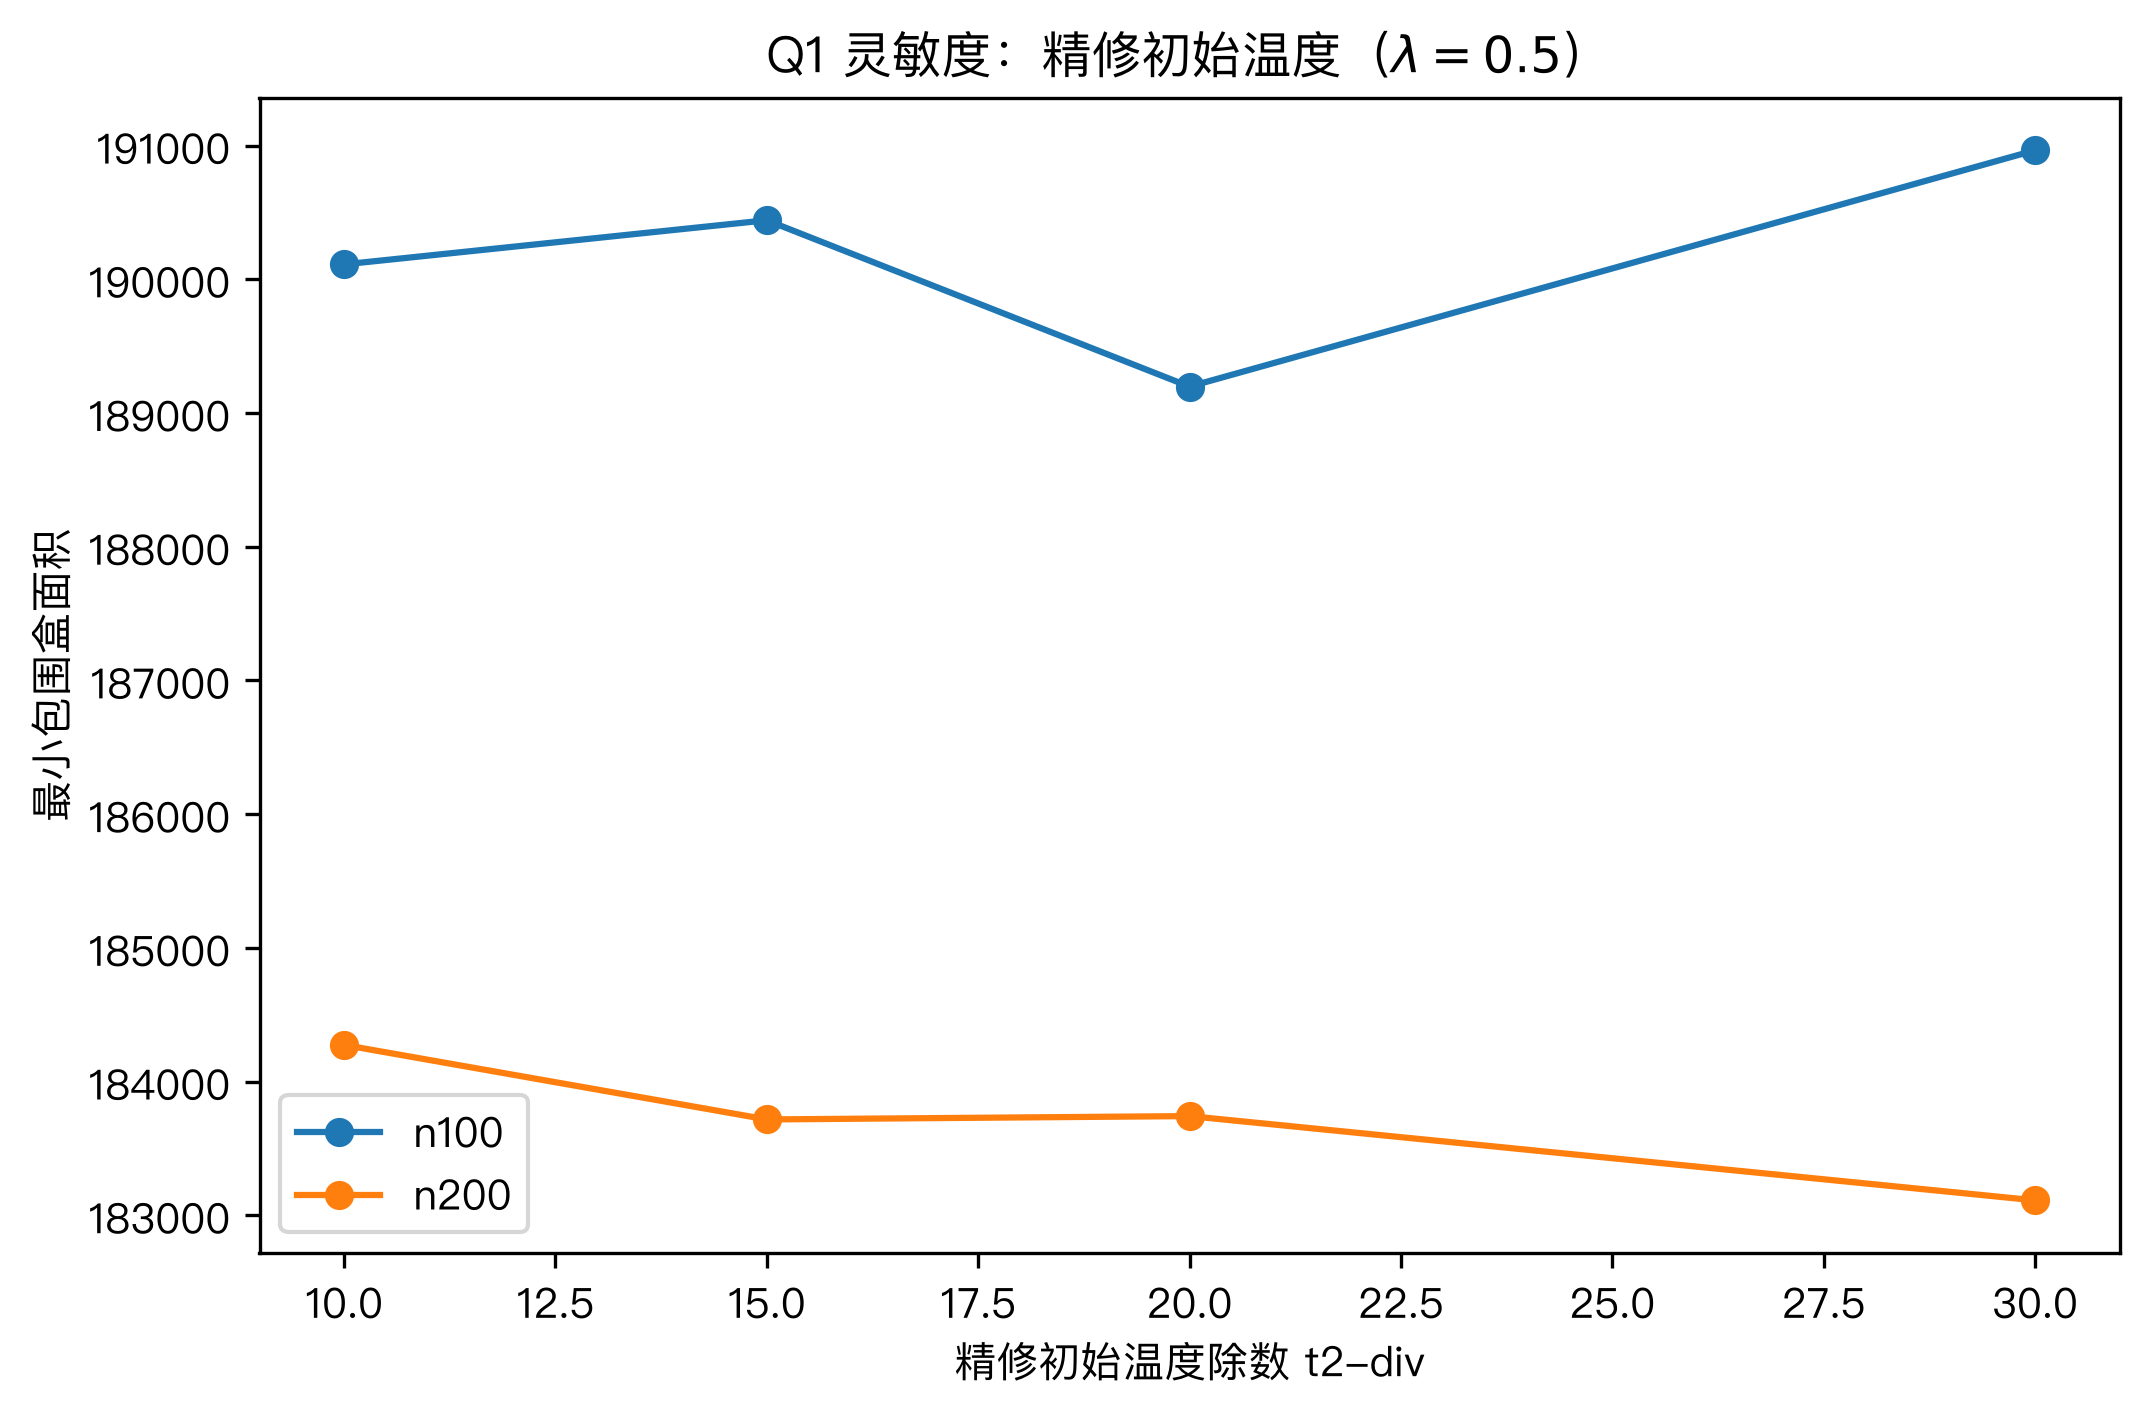
\includegraphics[width=0.82\textwidth]{../../图表/灵敏度/Q1/q1_t2div_sensitivity.png}
\caption{最优面积随精修温度除数变化}
\end{figure}

  \begin{table}[H]
  \centering
  \caption{S3 数据}\label{tab:q1s3}
  \begin{tabular}{llll}
  \toprule
  chip & t2\_div & area & aspect \\
  \midrule
  n100 & 10 & 190112 & 1.0986 \\
  n100 & 15 & 190442 & 1.0445 \\
  n100 & 20 & 189198 & 1.1039 \\
  n100 & 30 & 190965 & 1.0092 \\
  n200 & 10 & 184274 & 1.1633 \\
  n200 & 15 & 183717 & 1.0876 \\
  n200 & 20 & 183742 & 1.2592 \\
  n200 & 30 & 183112 & 1.2952 \\
  \bottomrule
  \end{tabular}
  \end{table}

\textbf{结论}：n100 在默认 t2-div$=20$ 处最优（189198）；n200 随
t2-div 增大单调改善（t2-div$=30$ 时 183112，低于默认 20 的
183742）——定稿对 n200 取 t2-div$=30$（较默认降面积 0.34\% 且
长宽比更优）；n300 保持默认 t2-div$=20$。t2-div 的加密扫描
（40/50/60）因赛程时间未执行，如实记录。

\end{document}
